\documentclass{article}
\usepackage{graphicx} % Required for inserting images
\usepackage{amsmath}
\usepackage[english, russian] {babel}
\usepackage[utf8]{inputenc}
\usepackage[T2A]{fontenc}
\usepackage{minted}
\usepackage{float}
\usepackage{amssymb}

\title{Формальные языки программирвонаия}
\author{silvia.lesnaia }
\date{February 2025}

\begin{document}

\maketitle


\textbf{13.02.25}
\section{Введение в компиляторы}
\section{Теория формальных языков и трансляций}
    \subsection{Введение в компиляторы}

    Языки высокого уровня

    \hspace{50mm} $\leftarrow$ Трансляторы(компиляторы)

    Ассемблеры

    Машинные языки
    \subsection{ВВЕДЕНИЕ}
    
\begin{figure}[H]
    \centering
    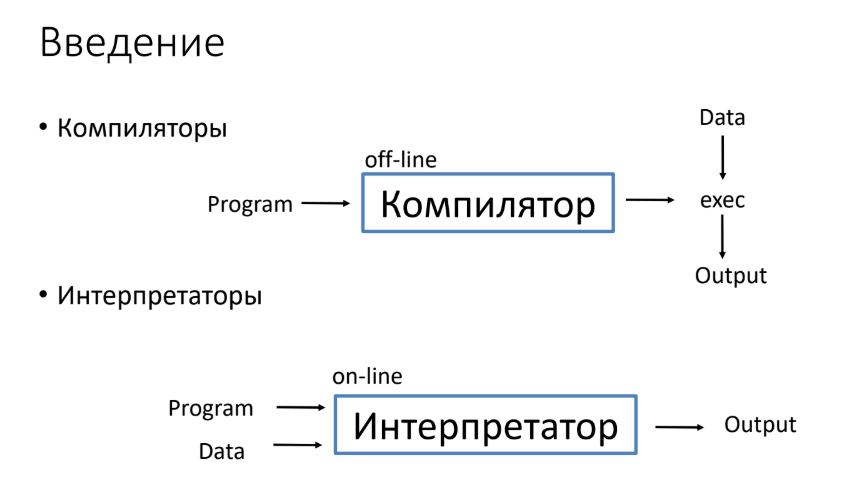
\includegraphics[width=1\linewidth]{Снимок экрана 2025-02-13 083445.png}
\end{figure}

    \subsubsection{Процесс компиляции}
    
    \begin{figure}[H]
        \centering
        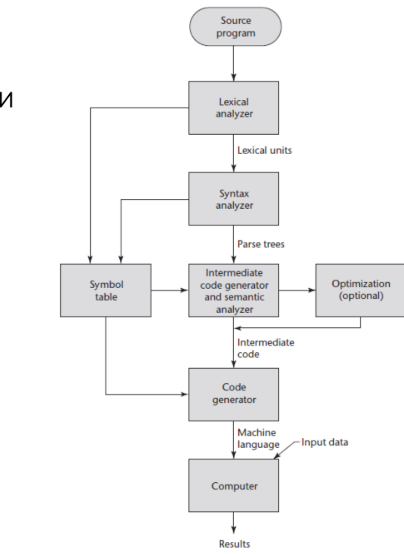
\includegraphics[width=1\linewidth]{Снимок экрана 2025-02-13 083723.png}
    \end{figure}

    \begin{figure}[H]
        \centering
        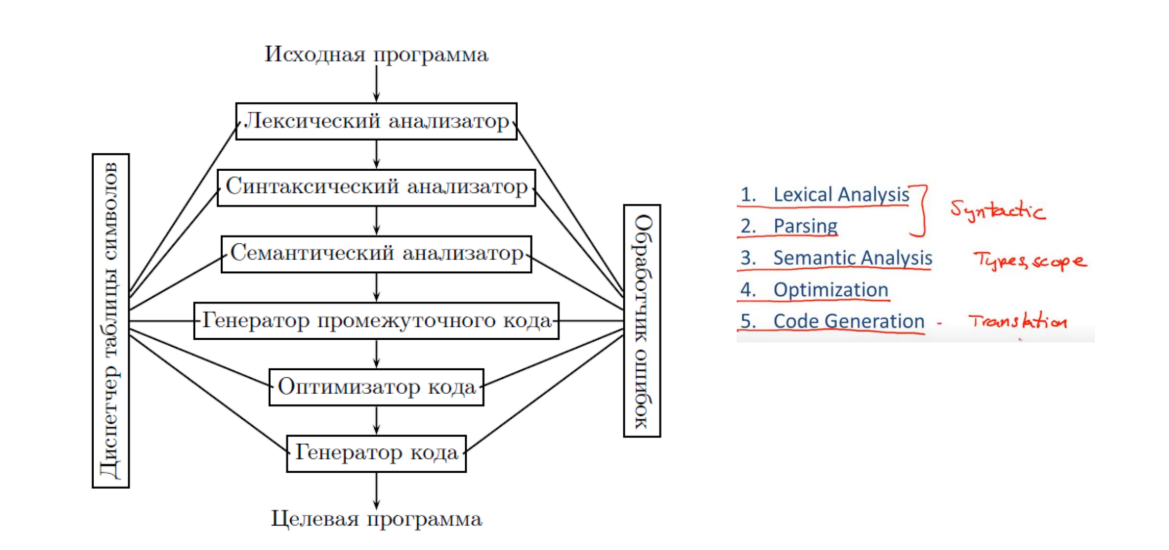
\includegraphics[width=1\linewidth]{Снимок экрана 2025-02-13 084306.png}
    \end{figure}

• 1. Лексический анализ – деление текста на слова, выделение
«токенов»

• This is a sentence

• Thi sis ase nte nce

• if x==y then z=1; else z=2;

\begin{figure}[H]
    \centering
    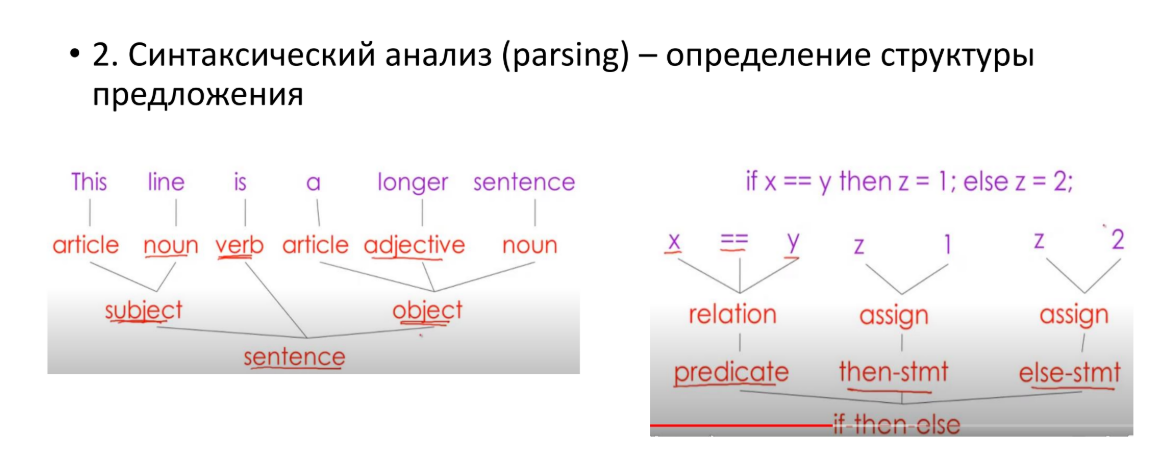
\includegraphics[width=1\linewidth]{Снимок экрана 2025-02-13 084508.png}
\end{figure}

• 3. Семантический анализ (устранение неоднозначностей)
• Пример:

• Петя сказал Мите оставить его задание дома

• Более сложный пример:

• Петя сказал Пете оставить его задание дома

• Языки программирования определяют строгие правила избегания
двусмысленности

{

int Jack = 3;

{

int Jack =4;

cout << Jack;

}

}

Компиляторы выполняют множество семантических проверок
относительно переменных

• Пример:

• Петя оставил её задание дома

• Из-за «несоответствия типов» между «её» и «Петя» мы узнаём,
что это разные люди.

• 4. Оптимизация кода

• На естественном языке оптимизация не имеет строгих правил и
сводится к редактированию.

• Для программы: Автоматическая модификация, чтобы:
• Работать быстрее

• Использовать меньше памяти

• (энергосбережение, сети, БД)

• X=Y*0

• X=0

• 5. Генерация кода

• Обычно результатом является ассемблерный код
или

• Трансляция на другой язык программирования

• Общая структура почти всех компиляторов соответствует нашему
описанию

• Пропорции в объеме вычислений в процессе трансляции
изменились:

\begin{figure}[H]
    \centering
    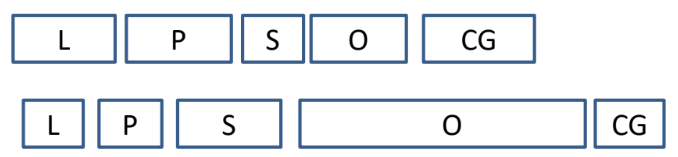
\includegraphics[width=0.5\linewidth]{Снимок экрана 2025-02-13 085253.png}
\end{figure}

\begin{figure}[H]
    \centering
    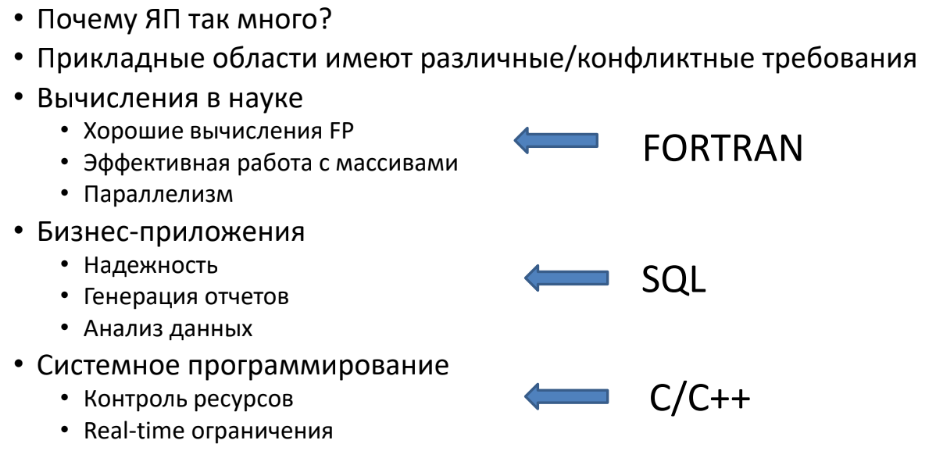
\includegraphics[width=1\linewidth]{Снимок экрана 2025-02-13 085330.png}
\end{figure}

\begin{figure}[H]
    \centering
    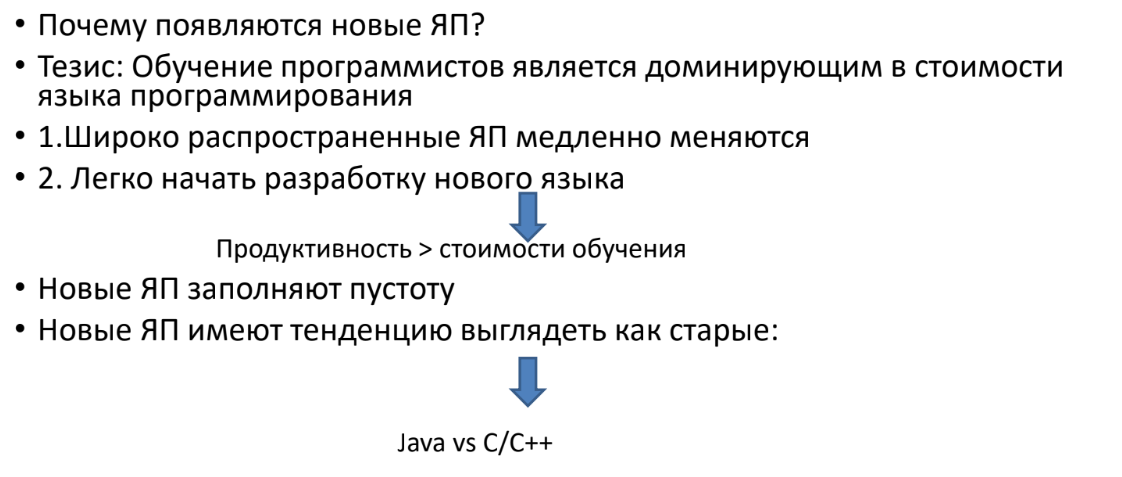
\includegraphics[width=1\linewidth]{Снимок экрана 2025-02-13 085352.png}
\end{figure}

\subsection{Лексический анализ}

• Просмотр потока символов программы (слева направо) и выделение
лексических единиц – токенов

position := initial + rate * 60

position – идентификатор

:= - операция

initial - идентификатор

+ - операция

rate - идентификатор

* - операция

60 - число (целое)

\begin{figure}[H]
    \centering
    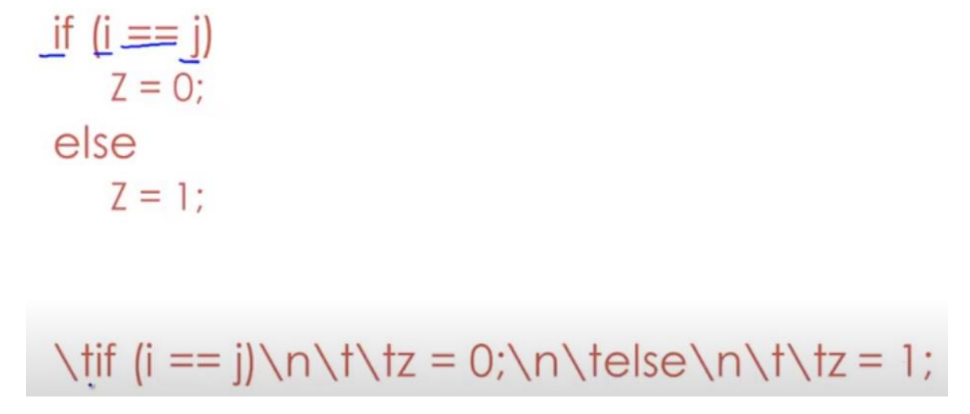
\includegraphics[width=1\linewidth]{Снимок экрана 2025-02-13 090554.png}
\end{figure}

• Классам токенов соответствуют множества строк
• Примеры:

• Идентификатор ::= строка букв и цифр, начинающаяся с буквы

• Целое число ::= непустая строка цифр

• Ключевое слово ::= < if | then | else | while | for | ...>

• Пробел ::= непустая последовательность кодов символов для
пробела новой строки, табуляции

\begin{figure}[H]
    \centering
    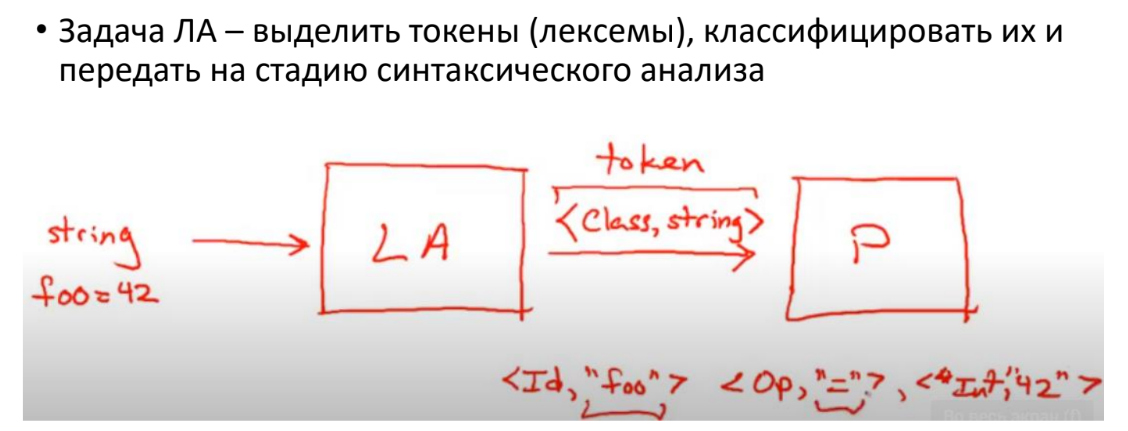
\includegraphics[width=1\linewidth]{Снимок экрана 2025-02-13 090702.png}
\end{figure}

if (i==j)

z=0;

else

z=1

\begin{figure}[H]
    \centering
    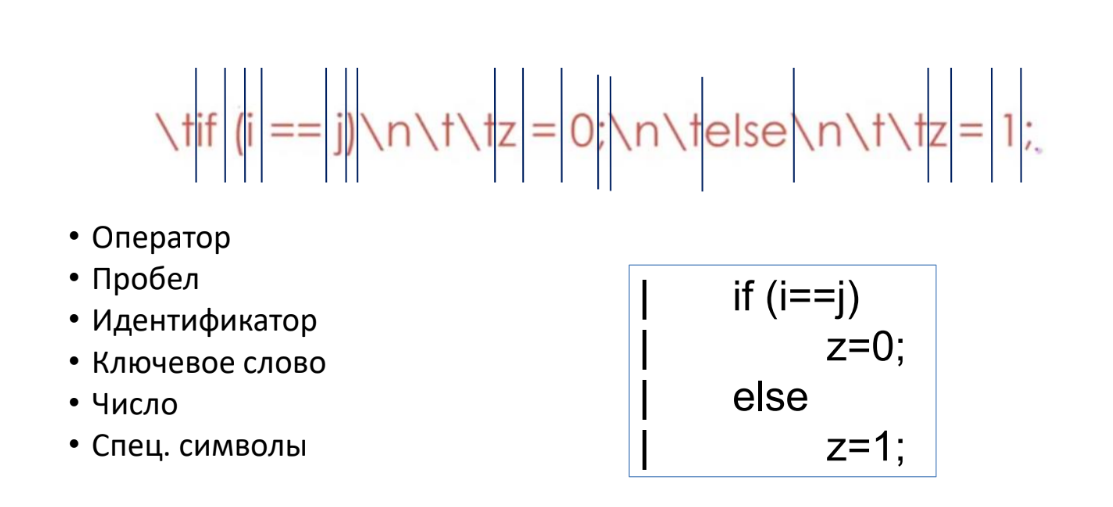
\includegraphics[width=1\linewidth]{Снимок экрана 2025-02-13 090834.png}
\end{figure}

• Примеры

• FORTRAN – пробелы не учитываются

• VAR1 – то же самое, что VA R1

• DO 5 i=1,25

• DO 5 i=1.25

• Необходимо заглядывать при просмотре строки вперёд

\begin{figure}[H]
    \centering
    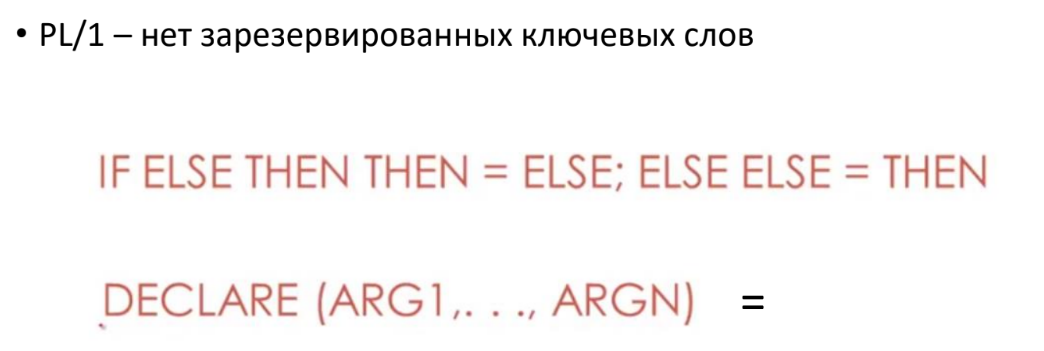
\includegraphics[width=1\linewidth]{Снимок экрана 2025-02-13 091234.png}
\end{figure}


• С++

• Синтакс :

• Foo<Bar>

• cin>>Bar

• Foo<Bar<Bazz>>

\subsection{Синтаксический анализ}

\begin{figure}[H]
    \centering
    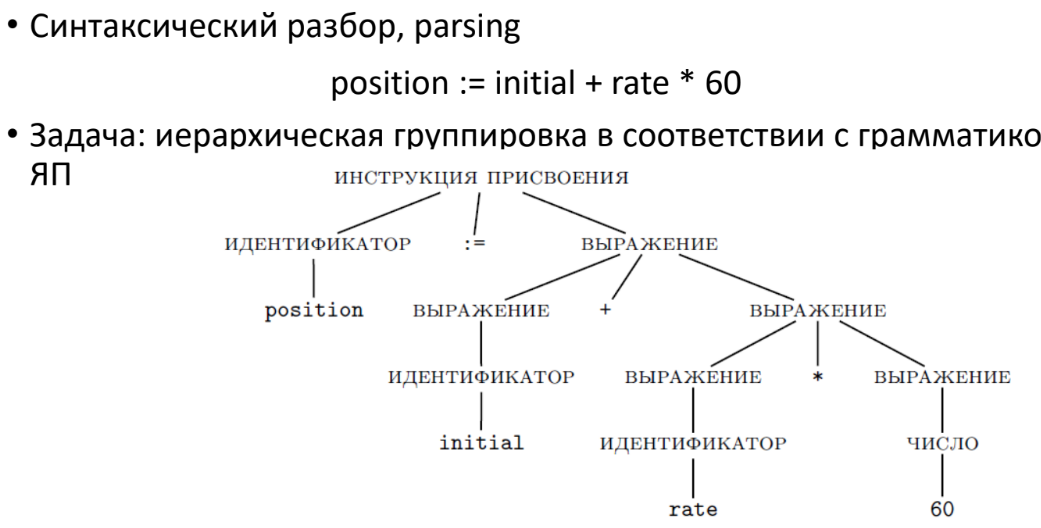
\includegraphics[width=1\linewidth]{Снимок экрана 2025-02-13 091654.png}
\end{figure}

\begin{figure}[H]
    \centering
    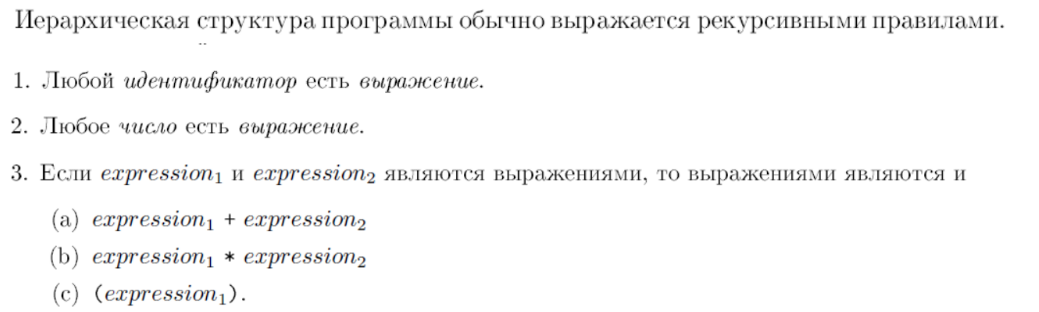
\includegraphics[width=1\linewidth]{Снимок экрана 2025-02-13 091754.png}
    \end{figure}
    
    \subsection{Семантический анализ}
    
\begin{figure}[H]
    \centering
    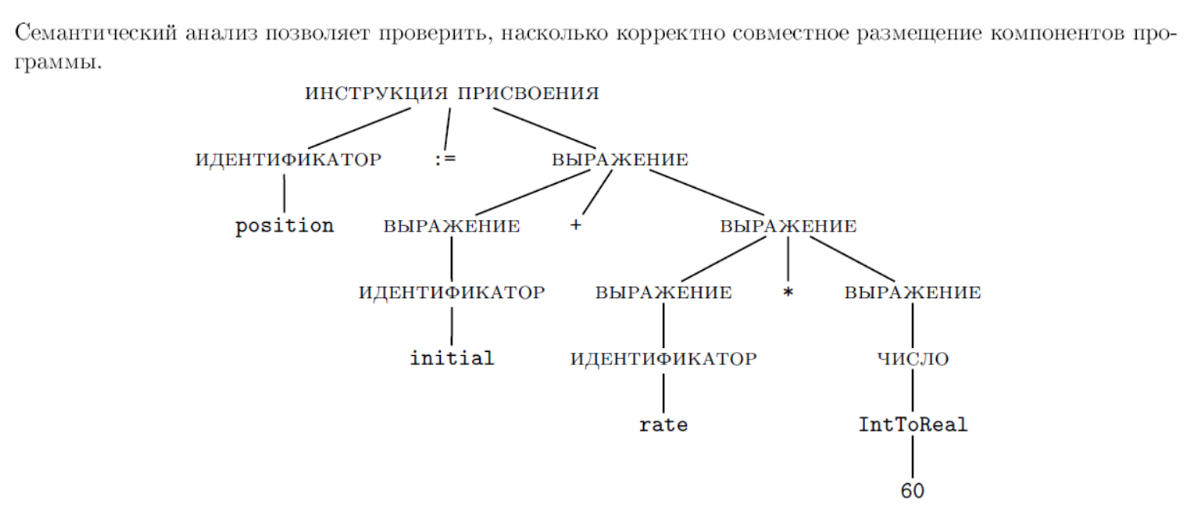
\includegraphics[width=1\linewidth]{Снимок экрана 2025-02-13 091809.png}
\end{figure}

\subsection{Генерация промежуточного кода}

\begin{figure}[H]
    \centering
    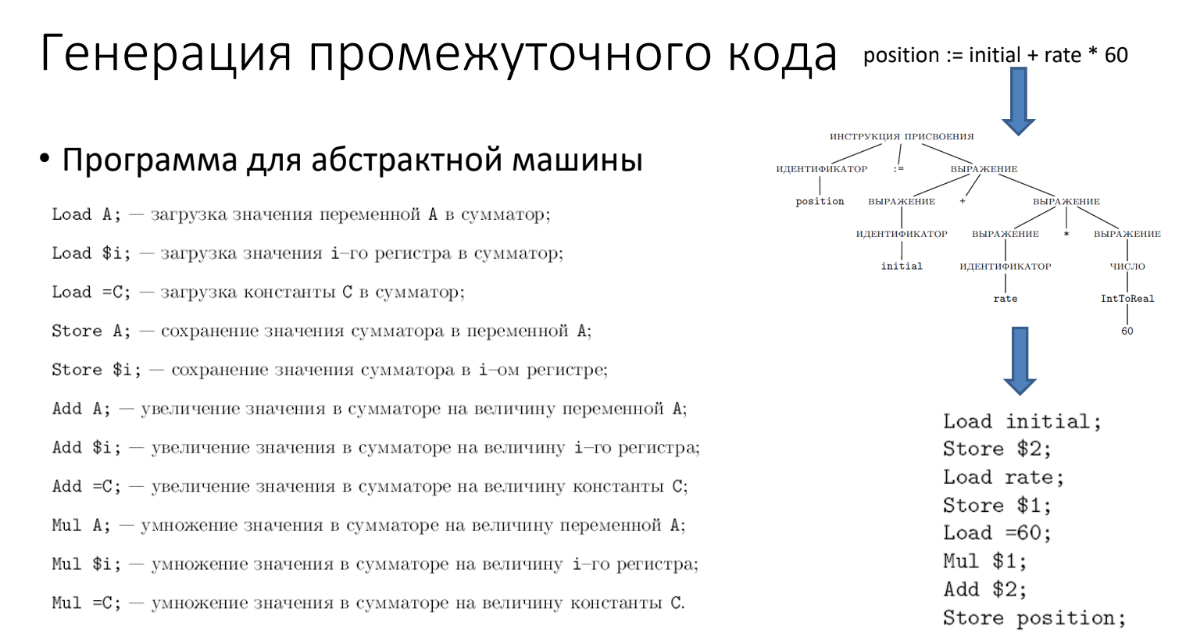
\includegraphics[width=1\linewidth]{Снимок экрана 2025-02-13 092347.png}
\end{figure}

\subsection{Зависимость от архитектуры компьютера}
\begin{figure}[H]
    \centering
    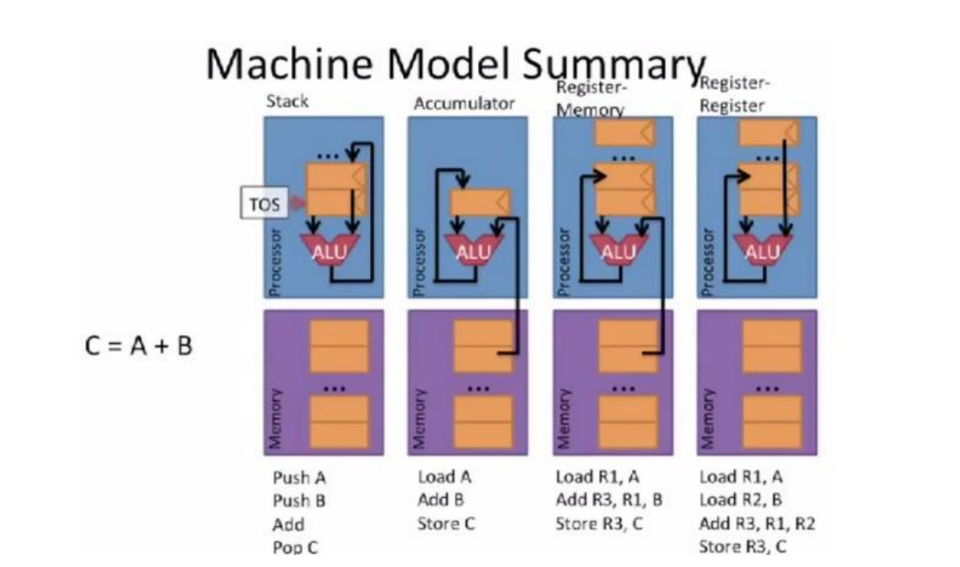
\includegraphics[width=1\linewidth]{Снимок экрана 2025-02-13 092401.png}
\end{figure}

\subsection{Оптимизация кода}

\begin{figure}[H]
    \centering
    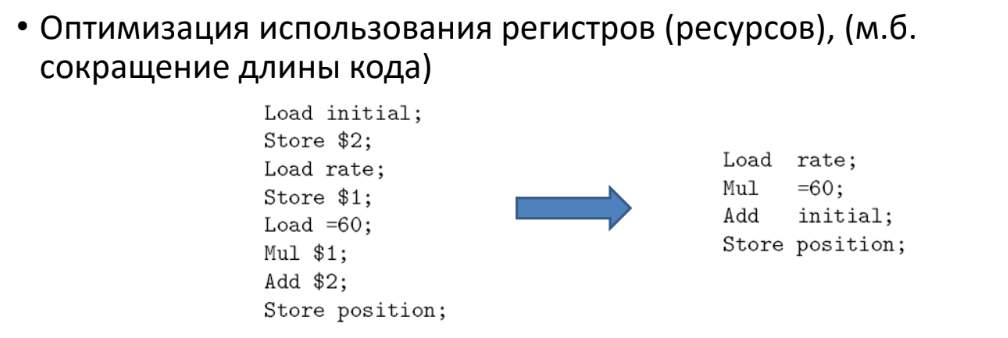
\includegraphics[width=1\linewidth]{Снимок экрана 2025-02-13 093155.png}
\end{figure}

\subsection{Генерация целевого кода}

\begin{figure}[H]
    \centering
    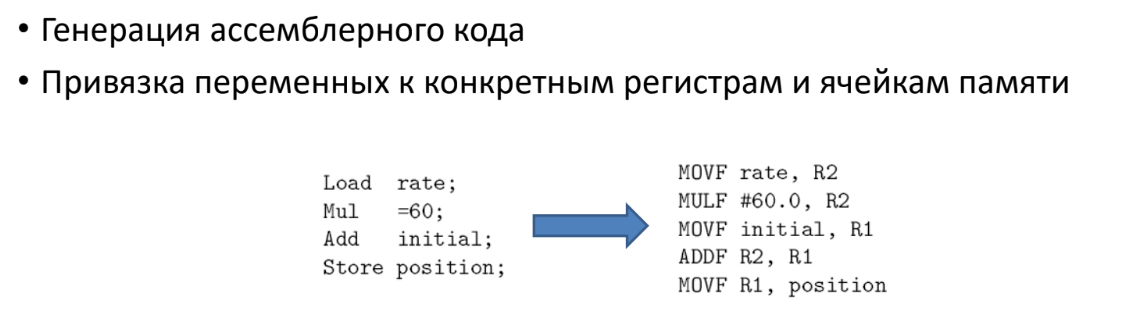
\includegraphics[width=1\linewidth]{Снимок экрана 2025-02-13 093218.png}
\end{figure}

\section{Формальные языки}

\subsection{Основные понятия и определения формальных языков}

• Опр. Алфавит — это конечное множество символов.

• Опр. Цепочкой символов (или словом) в алфавите $\Sigma$ называется любая конечная
последовательность символов этого алфавита.

• Опр. Цепочка, которая не содержит ни одного символа, называется пустой
цепочкой. Обозначение: $\epsilon$ (в алфавит $\Sigma$ не входит, она лишь помогает обозначить
пустую последовательность символов).

• Опр. Если a и b — цепочки, то цепочка ab (результат приписывания цепочки b в
конец цепочки a), называется конкатенацией (или сцеплением) цепочек a и b.
Конкатенацию можно считать двуместной операцией над цепочками: a×b = ab.

Например, если w = ab и z = cd, то w×z = abcd.

Для любой цепочки a : a$\epsilon$ = $\epsilon$a = a.

• Для любых цепочек a, b, g справедливо свойство ассоциативности операции конкатенации (ab)g = a(bg) = abg.

\subsection{Операции над цепочками символов}

\begin{figure}[H]
    \centering
    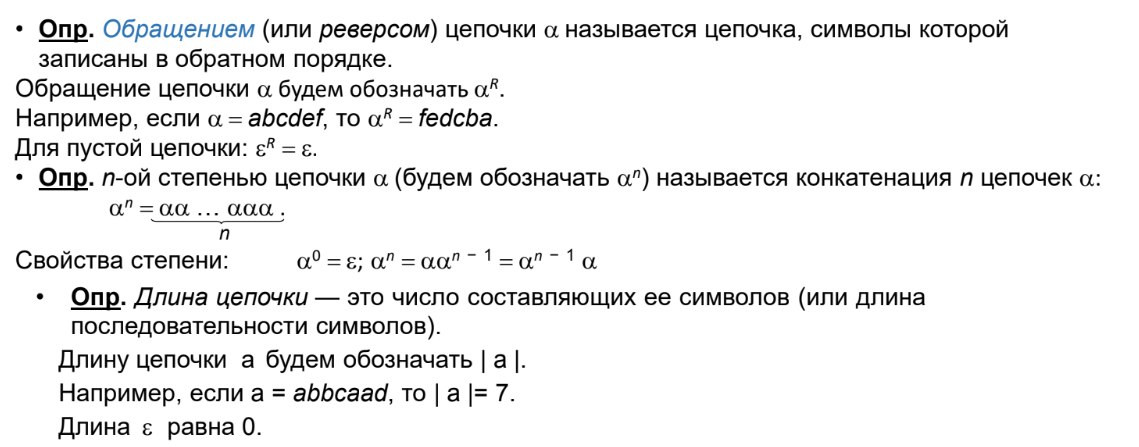
\includegraphics[width=1\linewidth]{Снимок экрана 2025-02-13 093643.png}
\end{figure}

\begin{figure}[H]
    \centering
    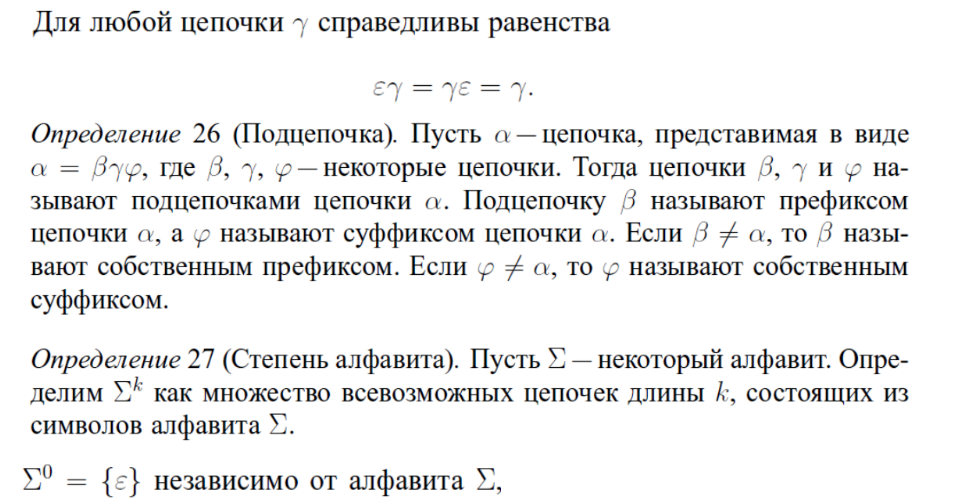
\includegraphics[width=1\linewidth]{Снимок экрана 2025-02-13 093853.png}
\end{figure}

\subsection{Формальный язык}
\begin{figure}[H]
    \centering
    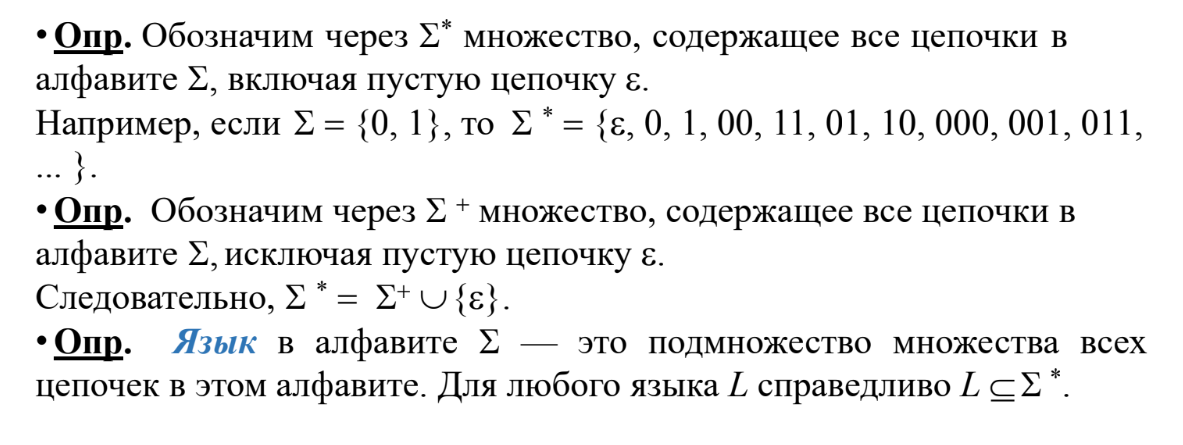
\includegraphics[width=1\linewidth]{Снимок экрана 2025-02-13 094552.png}
\end{figure}

\textbf{20.02.25}

\section{Формальный язык}


\begin{figure}[H]
    \centering
    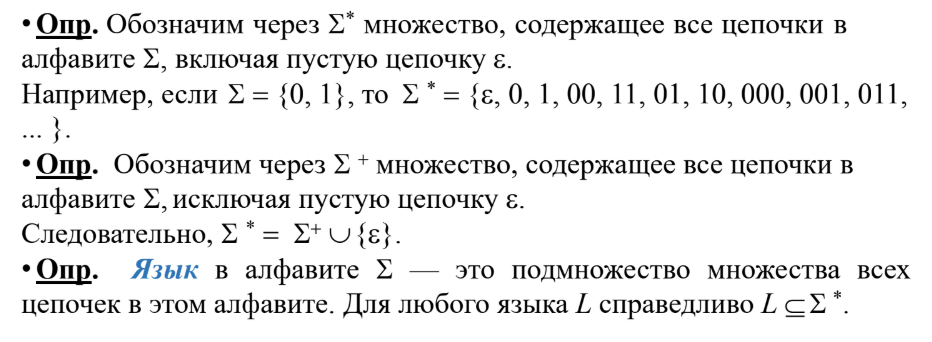
\includegraphics[width=1\linewidth]{image.png}
\end{figure}

Примеры

1. L = {$\varepsilon$, 01, 0011, 000111, 00001111, . . .} - язык над алфавитом
{0, 1}, в котором цепочки состоят из последовательностей k
единиц вслед за k нулями (k $\geq$ 0).
2. L = {$\varepsilon$}. Язык в любом алфавите, состоящий только из пустого
слова
3. L = $\varnothing$ Пустой язык в любом алфавите.
4. L = {$\varepsilon$, 01, 10, 0011, 1100, 1001, 0110, 0101, . . .} язык над
алфавитом {0, 1}, в котором равное число нулей и единиц.

\section{Операции над языками}
\begin{figure}[H]
    \centering
    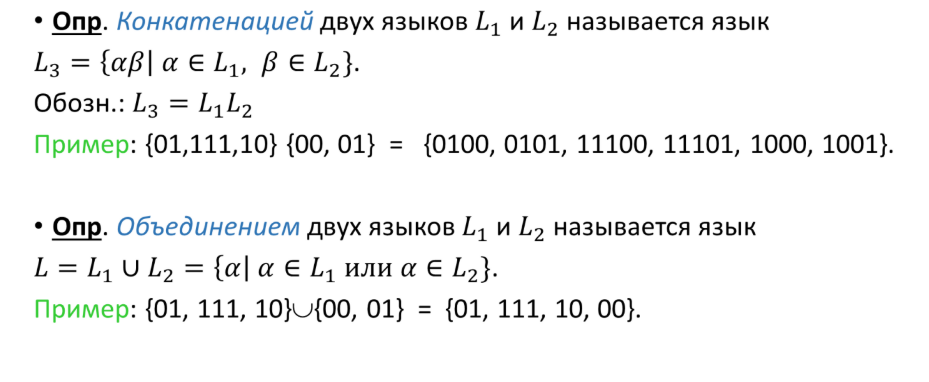
\includegraphics[width=1\linewidth]{Снимок экрана 2025-02-20 084202.png}
\end{figure}

\begin{figure}[H]
    \centering
    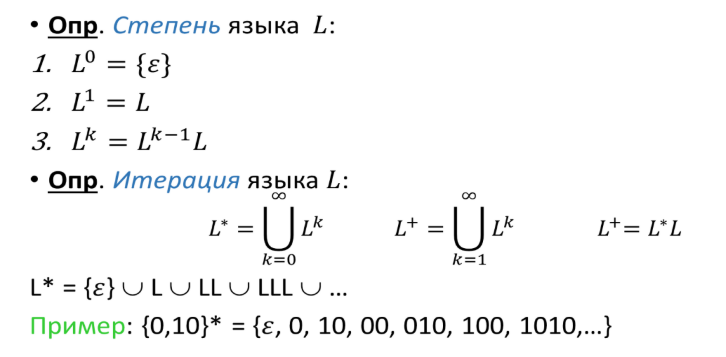
\includegraphics[width=1\linewidth]{Снимок экрана 2025-02-20 084233.png}
\end{figure}


\section{Способы описания языков}

• Конечный язык можно описать простым перечислением его
цепочек.

• Как представлять бесконечные языки?

• спецификация (описание)

• механизм распознавания

• механизм порождения (генерации).

• Не каждый формальный язык можно задать с помощью конечного
описания.


• Спецификация – Описание языка, как множества слов,
удовлетворяющих некоторому условию. (Для регулярных языков – это
регулярное выражение.

• Механизм распознавания (распознаватель), по сути, является
процедурой специального вида, которая по заданной цепочке
определяет, принадлежит ли она языку.

• Если принадлежит, то процедура останавливается с ответом «да», т. е.
допускает цепочку; иначе — останавливается с ответом «нет» или
зацикливается.

• Язык, определяемый распознавателем — это множество всех
цепочек, которые он допускает.

• Основной способ реализации механизма порождения —
использование порождающих грамматик

\section{Грамматики}

\begin{figure}[H]
    \centering
    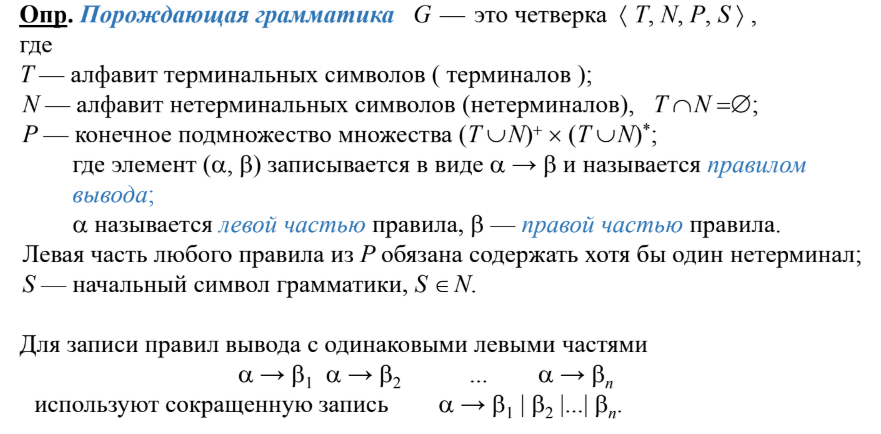
\includegraphics[width=1\linewidth]{Снимок экрана 2025-02-20 084954.png}
\end{figure}

Пример
$G_example$ = $\langle$ {0, 1}, {A, S}, P, S $\rangle$

P: S → 0A1

0A → 0A1

A → e

\section{Выводимость цепочки}

\begin{figure}[H]
    \centering
    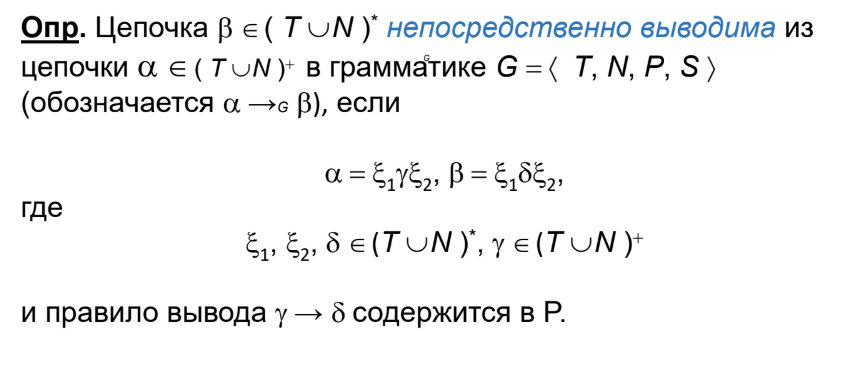
\includegraphics[width=1\linewidth]{Снимок экрана 2025-02-20 090552.png}
    
\end{figure}

\begin{figure}[H]
    \centering
    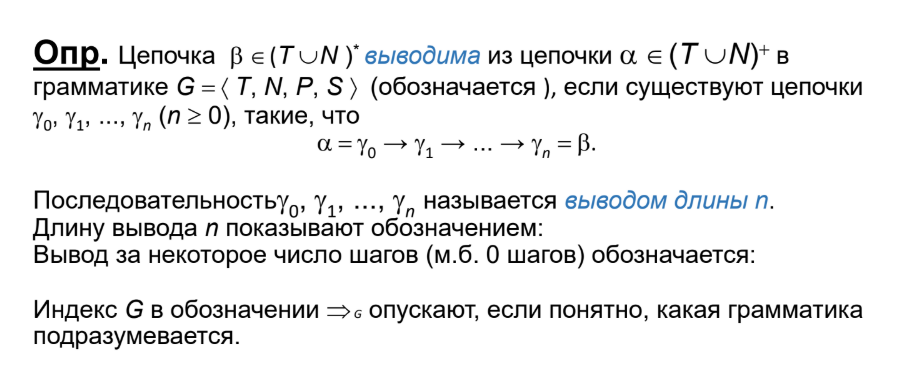
\includegraphics[width=1\linewidth]{Снимок экрана 2025-02-20 090612.png}
\end{figure}

\section{Язык грамматики}

\begin{figure} [H]
    \centering
    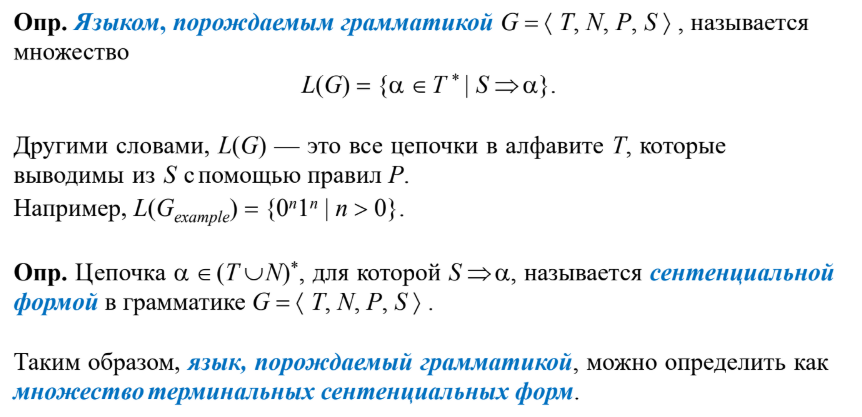
\includegraphics[width=1\linewidth]{Снимок экрана 2025-02-20 091501.png}
\end{figure}

\begin{figure}[H]
    \centering
    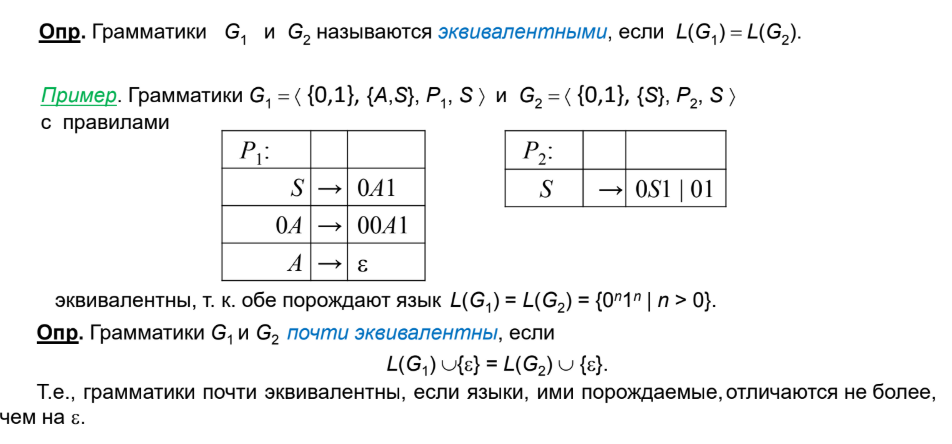
\includegraphics[width=1\linewidth]{Снимок экрана 2025-02-20 091507.png}
\end{figure}


\section{Распознаватель}
• Механизм, который является процедурой специального вида, которая по
заданной цепочке определяет, принадлежит ли она языку.

• Если принадлежит, то процедура останавливается с ответом «да», т. е.
допускает цепочку; иначе — останавливается с ответом «нет» или
зацикливается.

• Язык, определяемый распознавателем — это множество всех цепочек,
которые он допускает.

\begin{figure}[H]
    \centering
    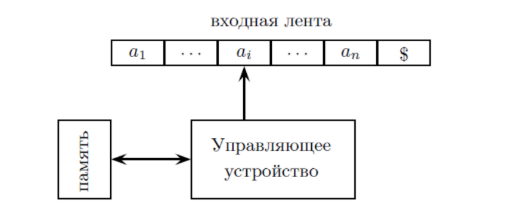
\includegraphics[width=0.5\linewidth]{Снимок экрана 2025-02-20 091653.png}
\end{figure}

\section{Классификация грамматик и языков по Хомскому}


• Тип грамматики определяется типом ограничений на вид
правил вывода.

• Всего определено четыре типа грамматик:
тип 0, тип 1, тип 2, тип 3.

• Каждому типу грамматик соответствует свой класс
языков.

• Если язык порождается грамматикой типа i (для i = 0, 1, 2,
3), то он является языком типа i.

\subsection{Классификация грамматик и языков по
Хомскому: Тип 0}

\textbf{Тип 0}

Любая порождающая грамматика является грамматикой
типа 0.

На вид правил грамматик этого типа не накладывается
никаких дополнительных ограничений.

Класс языков типа 0 совпадает с классом рекурсивно
перечислимых языков.

\subsection{Классификация грамматик и языков по
Хомскому: Тип 1}

Опр. Грамматика G = $\langle$ T, N, P, S $\rangle$ называется неукорачивающей, если
правая часть каждого правила из P не короче левой части (т. е. для
любого правила a → b $\epsilon$ P выполняется неравенство | a | $\leq$ | b | ).

В виде исключения в неукорачивающей грамматике допускается
наличие правила S → e, при условии, что S (начальный символ) не
встречается в правых частях правил.

Грамматикой типа 1 называют неукорачивающую грамматику.
\begin{figure}[H]
    \centering
    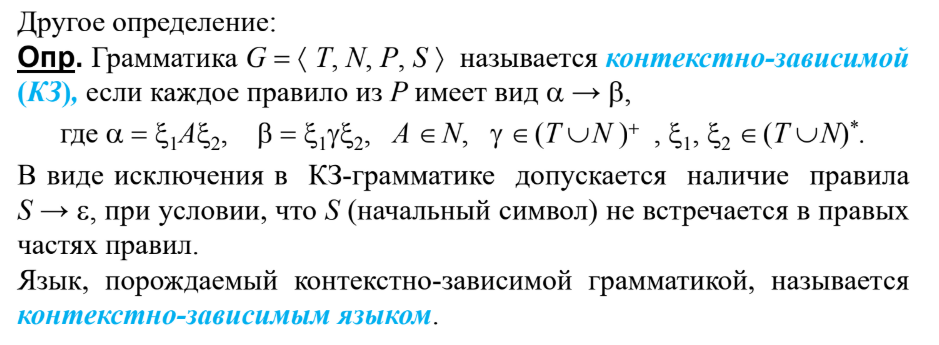
\includegraphics[width=1\linewidth]{Снимок экрана 2025-02-20 092937.png}
\end{figure}

\subsubsection{}{Эквивалентность неукорачивающих и
КЗ-грамматик}

Утверждение 1. Пусть L — формальный язык. Следующие утверждения
эквивалентны.
1) существует контекстно-зависимая грамматика $G_1$, такая что $L = L(G_1)$

2) существует неукорачивающая грамматика G2, такая что $L = L(G_2).$

Док-во. Очевидно, что (1) $\implies$ (2): любая контекстно-зависимая грамматика удовлетворяет ограничениям неукорачивающей грамматики (см. определения).

Т.к. каждое неукорачивающее правило можно заменить эквивалентной
серией контекстно-зависимых правил, следовательно (2) $\implies$ (1).

\subsection{Классификация грамматик и языков по
Хомскому: Тип 2}

Опр. Грамматика G = $\langle$ T, N, P, S $\rangle$ называется контекстно-свободной (КС),
если каждое правило из Р имеет вид A → b, где A $\varepsilon$N, b $\varepsilon$( T $\cup$ N )*.

Заметим, что в КС-грамматиках допускаются правила с пустыми правыми
частями. Язык, порождаемый контекстно-свободной грамматикой,
называется контекстно-свободным языком.
Грамматикой типа 2 будем называть контекстно-свободную грамматику.

КС-грамматика может являться неукорачивающей, т.е. удовлетворять
ограничениям неукорачивающей грамматики.

Утверждение 2. Для любой КС-грамматики G существует
неукорачивающая КС- грамматика G', такая что L(G) = L(G').

\subsection{Классификация грамматик и языков по
Хомскому: Тип 3}


\begin{figure}[H]
    \centering
    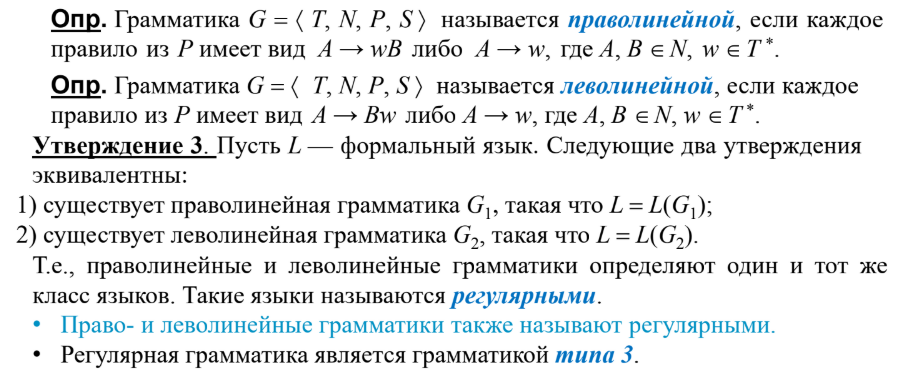
\includegraphics[width=1\linewidth]{Снимок экрана 2025-02-20 094134.png}
\end{figure}

\subsection{Автоматные грамматики}

Опр. Автоматной грамматикой называется праволинейная (леволинейная)
грамматика, такая, что каждое правило с непустой правой частью имеет вид:
A → a либо A → aB (для леволинейной, соответственно, A → a либо A → Ba),
где A, B $\epsilon$N, a $\epsilon$T.

Автоматная грамматика является более простой формой регулярной грамматики.

Существует алгоритм, позволяющий по регулярной (право- или леволинейной) грамматике построить соответствующую автоматную грамматику.

Таким образом, любой регулярный язык может быть порожден автоматной
грамматикой.

Существует алгоритм, позволяющий устранить из регулярной (автоматной)
грамматики все e-правила (кроме S → e в случае, если пустая цепочка принадлежит языку; при этом S не будет встречаться в правых частях правил).

Утверждение 4. Для любой регулярной (автоматной) грамматики G существует неукорачивающая регулярная (автоматная) грамматика G'
, такая что $L(G) = L(G')$.

\subsection{Иерархия грамматик Хомского}

Утверждение 5. Справедливы следующие утверждения:
1) любая регулярная грамматика является КС-грамматикой;
2) любая неукорачивающая КС-грамматика является КЗ-грамматикой;
3) любая неукорачивающая грамматика является грамматикой типа 0.

Утверждение 5 следует непосредственно из определений.

Рассматривая только неукорачивающие регулярные и неукорачивающие КС-
грамматики, получаем следующую иерархию классов грамматик:

Регулярные неукорачивающие $\subset$ КС неукорачивающие $\subset$ КЗ $\subset$ Тип 0

\section{Иерархия языков}

Утверждение 6. Справедливы следующие утверждения:
1) Каждый регулярный язык является КС-языком, но существуют КС-языки,
которые не являются регулярными, например:

$L = \{ a^n b^n | n  > 0 \}  $

2) Каждый КС-язык является КЗ-языком, но существуют КЗ-языки,
которыене являются КС-языками, например:

$ L = \{a^n b^n c^n | n > 0\}; $

3) Каждый КЗ-язык является языком типа 0 (т. е. рекурсивно перечислимым
языком), но существуют языки типа 0, которые не являются КЗ-языками.
Из утверждения 6 следует иерархия классов языков:

Тип 3 (Регулярные) $\subset$ Тип 2 (КС)  $\subset$ Тип 1 (КЗ)  $\subset$ Тип 0

\begin{figure}[H]
    \centering
    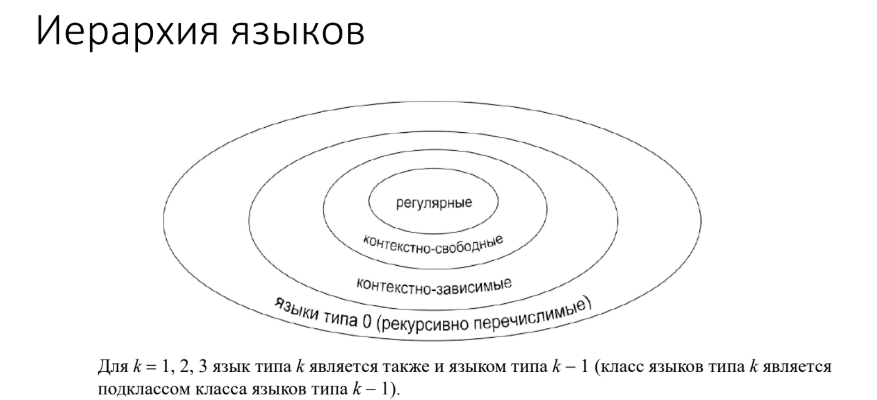
\includegraphics[width=1\linewidth]{Снимок экрана 2025-02-27 084055.png}
\end{figure}


• Утверждение 7. Проблема «Можно ли язык, описанный
грамматикой типа k (k = 0, 1, 2), описать грамматикой типа k + 1?»
является алгоритмически неразрешимой.

• Т.е., нет алгоритма, позволяющего по заданному описанию языка L
(например, по грамматике), определить максимальное k, такое что L
является языком типа k

• НО! В примерах и задачах при ответе на вопрос «Какого типа заданный
язык L?» будем указывать, если не оговорено иное, максимально
возможное k для заданного языка L.

\textbf{27.02.25}

\section{Разбор цепочек}

Опр. Цепочка в алфавите T принадлежит языку, порождаемому грамматикой
$ \langle  T, N, P, S \rangle $ , только в том случае, если существует ее вывод из начального
символа S этой грамматики.

• Процесс построения такого вывода (а, следовательно, и определения
принадлежности цепочки языку) называется разбором.
• Построение вывода можно осуществлять и в обратном порядке: в исходной
цепочке ищем вхождение в неё правой части некоторого правила и заменяем
егона левую часть (делаем свёртку).

• В итоге исходная цепочка «сворачивается» к некоторой сентенциальной
форме. Затем идет следующая свертка и т. д., пока не придем к S .
• Такой процесс разбора называют также анализом.

\begin{figure}[H]
    \centering
    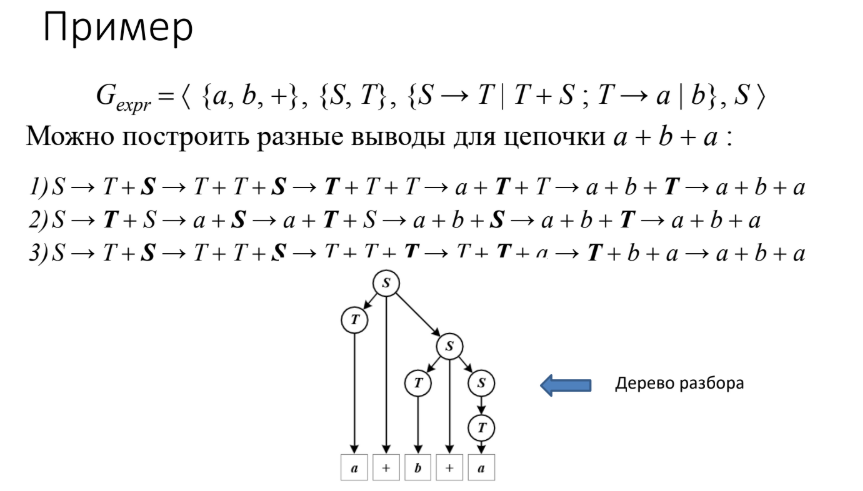
\includegraphics[width=1\linewidth]{Снимок экрана 2025-02-27 084444.png}
\end{figure}

\section{Регулярные множества, их распознавание и порождение}

\subsection{Регулярные множества и регулярные выражения}

• Опр. Пусть $\Sigma$ - конечный алфавит. Регулярное множество в
алфавите $\Sigma$ определяется следующим образом:
1) $\varnothing$ - регулярное множество в алфавите $\Sigma$.

2) $\{\epsilon\} $- регулярное множество в алфавите $\Sigma$.

3) $\{\alpha\}$ - регулярное множество в алфавите $\Sigma$ для каждого $\alpha \in  \Sigma$.

4) Если Q и P - регулярные множества в алфавите $\Sigma,$ то множества
Q $\cup$ P , QP и P* регулярные.

5) Ничто другое не является регулярным множеством в алфавите $\Sigma$.

\subsection{Регулярные выражения}


Опр. Пусть $\Sigma$ — конечный алфавит. Определим рекурсивно регулярное
выражение в алфавите $\Sigma$ и регулярные множества, которые они обозначают.
Базис индукции:

1) $\varnothing$ есть регулярное выражение, обозначающее регулярное множество $\varnothing$

2) $\epsilon$ есть регулярное выражение, обозначающее регулярное множество $\{\epsilon\} $

3) $\alpha \in \Sigma$  есть регулярное выражение, обозначающее регулярное множество $\{\alpha\}$
Индукция:

Если $\alpha$ и $\beta$ — регулярные выражения, обозначающие регулярные множества Q$\cup $P соответственно, то:

1) ($\alpha + \beta $) — регулярное выражение, обозначающее Q$\cup$P;

2) ($\alpha \beta $) — регулярное выражение, обозначающее QP;

3) ($\beta$)*

* — регулярное выражение, обозначающее P*;

Никаких других регулярных выражений, кроме тех, что построены в
соответствии с описанным определением, нет.


\begin{figure}[H]
    \centering
    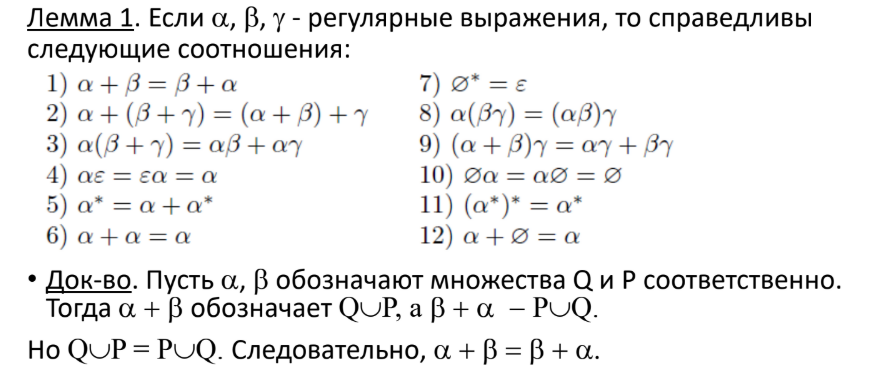
\includegraphics[width=1\linewidth]{Снимок экрана 2025-02-27 085900.png}
\end{figure}



\subsection{Алгебраические законы для регулярных
выражений}
• Объединение и конкатенация ведут себя как сложение и
умножение.

• + является коммутативным и ассоциативным;

• Конкатенация является ассоциативной операцией.

• Конкатенация распределяется по +.

• Исключение: Конкатенация не коммутативна.

\subsection{Единицы и нейтральные элементы в RE}

• $\varnothing$ является нейтральным элементом для +.
R + $\varnothing$ = R.

• e является «единицей» для конкатенации.
$\epsilon R = R\epsilon = R.$

• $\varnothing $ является «нулем» для конкатенации.
$\varnothing R = R \varnothing = \varnothing.$

\textbf{Пример преобразования RE}

!ЭТА ЗАДАЧА БУДЕТ В кр

\begin{figure}[H]
    \centering
    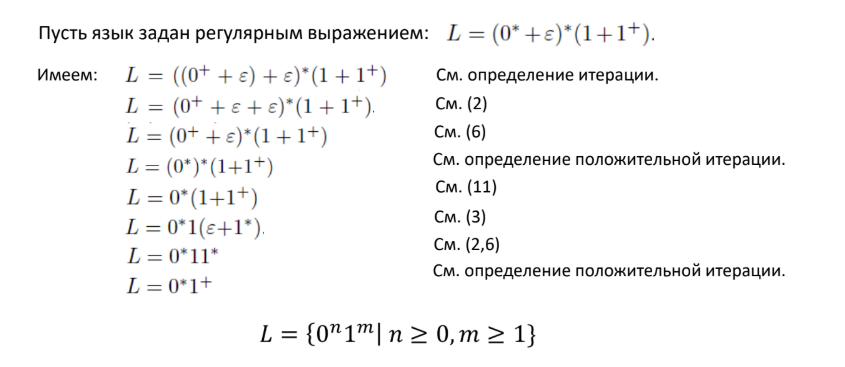
\includegraphics[width=1\linewidth]{Снимок экрана 2025-02-27 090738.png}
\end{figure}


\textbf{Примеры RE}


• $\Sigma=\{0,1\}$

• $ L(01) = \{01\}.$

• $L(01+0) = \{01, 0\}.$

• $L(0(1+0)) = \{01, 00\}.$

• $ L(0*) = \{\epsilon, 0, 00, 000,... \}.$

• $ L((0+10)*(\epsilon+1))$ = все строки из 0 и 1 без двух последовательных 1.
 

\begin{figure}[H]
    \centering
    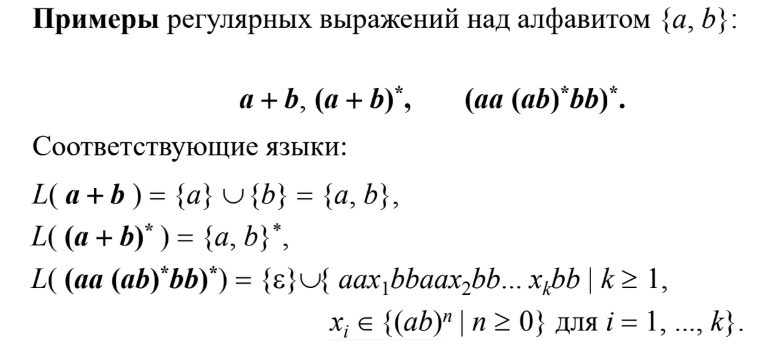
\includegraphics[width=1\linewidth]{Снимок экрана 2025-02-27 091410.png}
\end{figure}

\subsection{Уравнения с регулярными коэффициентами}

• Рассм. уравнение X=aX+b, где a и b – РВ.
X=a*b – решение уравнения:

a*b=aa*b+b

a*b=(aa*+e)b

a*b=a*b

Если множество, определяемое рег. выражением a, содержит e, то
ур-е имеет бесконечно много решений: X=a*(b+c) для любого РВ c.
В этом случае берут «наименьшее решение» – наименьшую
неподвижную точку.

\end{document}
